\documentclass[wide,a4paper,titlepage,12pt] {article}
\usepackage{polski}
\usepackage[utf8]{inputenc}
\usepackage{placeins}
\usepackage{longtable}
\usepackage{graphicx}
\usepackage{xcolor,listings}



\title{Inżynieria e-systemów java}
\author{Tymon Tobolski (181037)\\ Jacek Wieczorek (181043) \\ Mateusz Lenik(181142)}

% Title page layout (fold)
\makeatletter
\renewcommand{\maketitle}{
\begin{titlepage}
  \begin{center}
    \vspace*{3cm}
    \LARGE \@title \par
    \vspace{2cm}
    \textit{\small Autor:}\par
    \normalsize \@author\par \normalsize
    \vspace{3cm}
    \textit{\small Prowadzący:}\par
    Dr inż. Katarzyna Nowak \par
    \vspace{2cm}
    Wydział Elektroniki\\ III rok\\ Śr 7.30 - 9.00\par

  \end{center}
\end{titlepage}
}


\begin{document}
  \maketitle
  \tableofcontents
  \newpage

  \section{Opis projektu}
  \paragraph{}
  Celem projektu jest stworzenie portalu, pozwalającego użytkownikowi na zakładanie i prowadzenie mikroblogów wraz zmożliwością follow'ania wpisów innych użytkowników. Aplikacja zostałą napisana w języku ruby z wykorzystaniem framework'a Ruby on Rails.
  \begin{itemize}
    \item Platforma : JVM
    \item Język impementacji : ruby, coffescript
    \item Framework : Ruby on Rails 
  \end{itemize}
  \section{Funkcjonalności systemu}
  \paragraph{}
  \begin{itemize}
   \item Obsługa użytkowników
   \begin{itemize}
    \item Tworzenie konta
    \item Edycja użytkownika
    \item System autentykacji
    \item Usuwanie użytkowników
    \item Follow user
   \end{itemize}
   \item Obsługa blogów
    \begin{itemize}
      \item Tworzenie bloga
      \item Zarządzanie blogiem
      \item Tablica z postami użytkowników "follow"
    \end{itemize}
   \item Obsługa postów
    \begin{itemize}
      \item Dodawanie posta
      \item Usuwanie posta
    \end{itemize}
  \item Dyskusje
    \begin{itemize}
      \item Tworzenie dyskusji
      \item Zarządzanie dyskusjami
      \item Dyskusje publiczne i prywatne
      \item Zapraszanie użytkowników
      \item Dodawanie postów w dyskusji
    \end{itemize}
  \item Dodatkowe funkcjonalności
    \begin{itemize}
      \item Powiązanie kont użytkowników z kontami facebook (logowanie przy użyciu facebook'a)
      \item Pobieranie avatarów z gravatara
    \end{itemize}
  \end{itemize}
  \section{Implementacja}
  \paragraph{}
  System został zaimplementowany w architekturze $MVC$ z wykorzystaniem architektury $REST$.
  \subsection{Kontrolery}
    \subsubsection{Blogs Controller}
    \paragraph{}
      Kontroler odpowiadający za funkcjonalności blogów : tworzenie, edytowanie, usuwanie, wyświetlanie, zabezpieczenie dostępu do edycji osób nie mających odpowiednich uprawnień.
    \subsubsection{Home Conroller}
    \paragraph{} % (fold)
    \label{par:}
    Kontroler odpowiadający za wyświetlanei stron statycznych np : About, Contact, etc. 
    % paragraph  (end)
    \subsubsection{Invitations Controller}
    \paragraph{}
    Kontroler odpowiedzialny za dodawanie i usuwanie użytkowników z dyskusji.

    \subsubsection{OmniauthCallbacks Controller}
    \paragraph{}
    Kontroler odpowiedzialny za możliwość logowania się przez konto Facebook.
    
    \subsubsection{Posts Controller}
    \paragraph{}
    Kontroler odpowiedzialny za funkcjonalnośći postów.
    
    \subsubsection{Registration Controller}
    \paragraph{}
    Kontroler odpowiedzialny za niestandardowe przeładowanie po rejestracji użytkownika.
    
    \subsubsection{Relationships Controller}
    \paragraph{}
    Kontroler odpowiedzialny za akcje typu Follow/Unfollow user.

    \subsubsection{Sessions Controller}
    \paragraph{}
    Kontroler odpowiedzialny za edycję profilu użytkownika

    \subsubsection{Inne}
    \paragraph{}
    W celu stowrzenia systemu atentykacji i rejestracji użytkowników skorzystaliśmy z gotowej biblioteki \textit{Devise}. Wszelkie dodatkowe akcje zawarte w kotrolerach : Session, Registration i OmniauthCallbacks pozwalają nam na dostosowanie systemu do naszych potrzeb w szybki i wygodny sposób.

    \subsection{Views}
    \paragraph{}
    Wszelkei widoki zostały napisane przy uzyciu języka znaczników \textit{Haml}. W celu generowania formularzy użyty został gem \textit{SimpleForm}, a cały layout oparty o bibliotekę styli css - \textit{Bootstrap}. Skrypty wykorzystujące \textit{jQuery}, napisane zostały przy pomocy języka \textit{CoffeScript}, kompilowalnego do kodu javascript.

    \paragraph{}
    Wykorzystane biblioteki js i css :
    \begin{itemize}
      \item bootstrap css
      \item bootstrap tabs
      \item facebox
      \item jQuery
      \item jQuery ui
    \end{itemize}
    
    \subsection{Model}
    \paragraph{}
    W projekcie wykorzystana została baza danych \textit{PostgreSql} w wersji produkcyjnej i \textit{SqlLite} w wersji deweloperskiej.

    \paragraph{}
    W celu łatwego dostepu do bazy danych i zarządzania nimi skorzystalimy z biblioteki \textit{ActiveRecords} implementującej \textit{ORM}.

    \paragraph{}
    W projekcie wystpują następujące modele :
    \begin{itemize}
      \item Blog
      \item Invitation
      \item Post
      \item Relationship
      \item User
    \end{itemize}

      \begin{figure}[h!]
        \begin{center}
          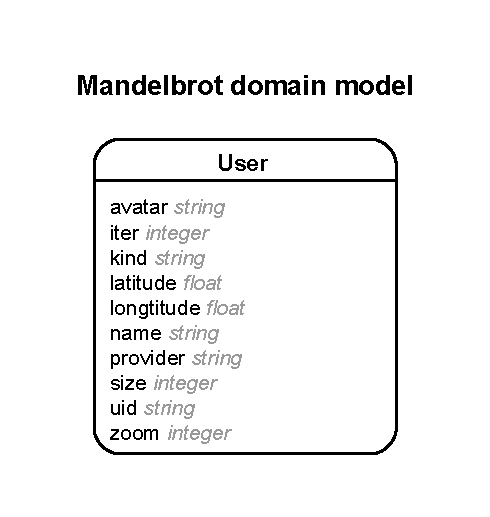
\includegraphics[scale=0.8]{erd.pdf}
        \end{center}
        \caption{Diagram ERD modelu}
        \label{fig:model}
      \end{figure}
      \newpage

      \newpage
      \subsection{Najważniejsze biblioteki}
      \paragraph{}
      \small{
        
\begin{lstlisting}[
    caption=Spis najważniejszych bibliotek,
    firstnumber=1,
    language=Ruby,
    keywordstyle=\color{red},
    stringstyle=\color{blue},
]
source 'https://rubygems.org'

gem 'rails', '3.2.2'

group :development do
  # gem do obslugi bazy danych sqlite
  gem 'sqlite3', :platform => :ruby 
  # gem do obslugi bazy danych sqlite jruby
  gem 'activerecord-jdbcsqlite3-adapter', :platform => :jruby 
  # generowanie diagramow
  gem "rails-erd" 
end

group :production do
  # gem do obslugi bazy danych Postgres
  gem 'pg', '0.12.2' 
end

...
# gem do obslugi autentykacji uzytkownikow
gem 'devise' 
# gem do obslugi logowania przez FB przy pomocy OAuth
gem 'omniauth-facebook' 
# gem pozwaljacy na wykorzystanie jezyka znacznikow HAML
gem 'haml' 
gem 'haml-rails'
# gem pozwalajacy na proste tworzenie formularzy
gem 'simple_form' 


group :assets do
  ...
  # gem pozwalajacy na pisanie javascript w jezyku CoffeScript
  gem 'coffee-rails' 
end

gem 'jquery-rails' # dolaczenie biblioteki js jQuery
gem 'jqueryui_rails' # dolaczenie biblioteki js jQuery-ui

\end{lstlisting}






      }

      \newpage
      \subsection{Routes}
      \paragraph{}
        \small{
            \tiny{
  \begin{center}
    \begin{longtable}{|c|c|c|c|}
    \hline
    Path name &Method & Path & Action \\ \hline

                    root &       &$/$                                        & home\#index \\
        new\_user\_session &GET    &$/$users$/$sign\_in(.:format)                  &devise$/$sessions\#new\\
            user\_session &POST   &$$/$$users$/$sign\_in(.:format)                 & devise$/$sessions\#create\\
    destroy\_user\_session &DELETE &$/$users$/$sign\_out(.:format)                & devise$/$sessions\#destroy\\
  user\_omniauth\_callback &       &$/$users$/$auth$/$:action$/$callback(.:format)   & omniauth\_callbacks\#(?-mix:facebook)\\
           user\_password &POST   &$/$users$/$password(.:format)                & devise$/$passwords\#create\\
       new\_user\_password &GET    &$/$users$/$password$/$new(.:format)            & devise$/$passwords\#new\\
      edit\_user\_password &GET    &$/$users$/$password$/$edit(.:format)           & devise$/$passwords\#edit\\
                         &PUT    &$/$users$/$password(.:format)                & devise$/$passwords\#update\\
cancel\_user\_registration &GET    &$/$users$/$cancel(.:format)                  & registrations\#cancel\\
       user\_registration &POST   &$/$users(.:format)                         & registrations\#create\\
   new\_user\_registration &GET    &$/$users$/$sign\_up(.:format)                 & registrations\#new\\
  edit\_user\_registration &GET    &$/$users$/$edit(.:format)                    & registrations\#edit\\
                         &PUT    &$/$users(.:format)                         & registrations\#update\\
                         &DELETE &$/$users(.:format)                         & registrations\#destroy\\
                 profile &GET    &$/$profile$/$:id(.:format)                   & sessions\#show\_profile\\
            edit\_profile &GET    &$/$profile$/$:id$/$edit(.:format)              & sessions\#edit\_profile\\
                 profile &PUT    &$/$profile$/$:id(.:format)                   & sessions\#update\_profile\\
               following &GET    &$/$profile$/$:id$/$following(.:format)         & sessions\#following\\
               followers &GET    &$/$profile$/$:id$/$followers(.:format)         & sessions\#followers\\
           delte\_profile &DELETE &$/$profile$/$:id$/$delete(.:format)            & sessions\#delete\_profile\\
              blog\_posts &POST   &$/$blogs$/$:blog\_id$/$posts(.:format)          & posts\#create\\
               blog\_post &DELETE &$/$blogs$/$:blog\_id$/$posts$/$:id(.:format)      & posts\#destroy\\
        blog\_invitations &POST   &$/$blogs$/$:blog\_id$/$invitations(.:format)     &invitations\#create\\
         blog\_invitation &DELETE &$/$blogs$/$:blog\_id$/$invitations$/$:id(.:format) &invitations\#destroy\\
                   blogs &GET    &$/$blogs(.:format)                          &blogs\#index\\
                         &POST   &$/$blogs(.:format)                          &blogs\#create\\
                new\_blog &GET    &$/$blogs$/$new(.:format)                      &blogs\#new\\
               edit\_blog &GET    &$/$blogs$/$:id$/$edit(.:format)                 &blogs\#edit\\
                    blog &GET    &$/$blogs$/$:id(.:format)                      &blogs\#show\\
                         &PUT    &$/$blogs$/$:id(.:format)                      &blogs\#update\\
                         &DELETE &$/$blogs$/$:id(.:format)                     & blogs\#destroy\\
           relationships &POST   &$/$relationships(.:format)                 & relationships\#create\\
            relationship &DELETE &$/$relationships$/$:id(.:format)             & relationships\#destroy\\
                    help &       &$/$help(.:format)                          & home\#help\\
                   about &       &$/$about(.:format)                         & home\#about\\
                 contact &       &$/$contact(.:format)                       & home\#contact\\
                userlist &       &$/$userlist(.:format)                      & home\#user\_list\\
            unauthorized &       &$/$unauthorized(.:format)                  & home\#unauthorized\\ \hline

\caption{Ścieżki dostępne w aplikacji}\\
    \end{longtable}
\end{center}
}
        }


      \section{Testy}
      \paragraph{}
      TODO




  
\end{document}